\section{Definition der Anlagenkomponenten} \label{Anlagenkomponenten}
	Die allgemeine Kommunikationstopologie (\ref{fig:Kommunikationstopologie}) der funktionsrelevanten Komponenten sieht wie folgt aus: 
	
	\begin{figure}[h!]
		\centering
		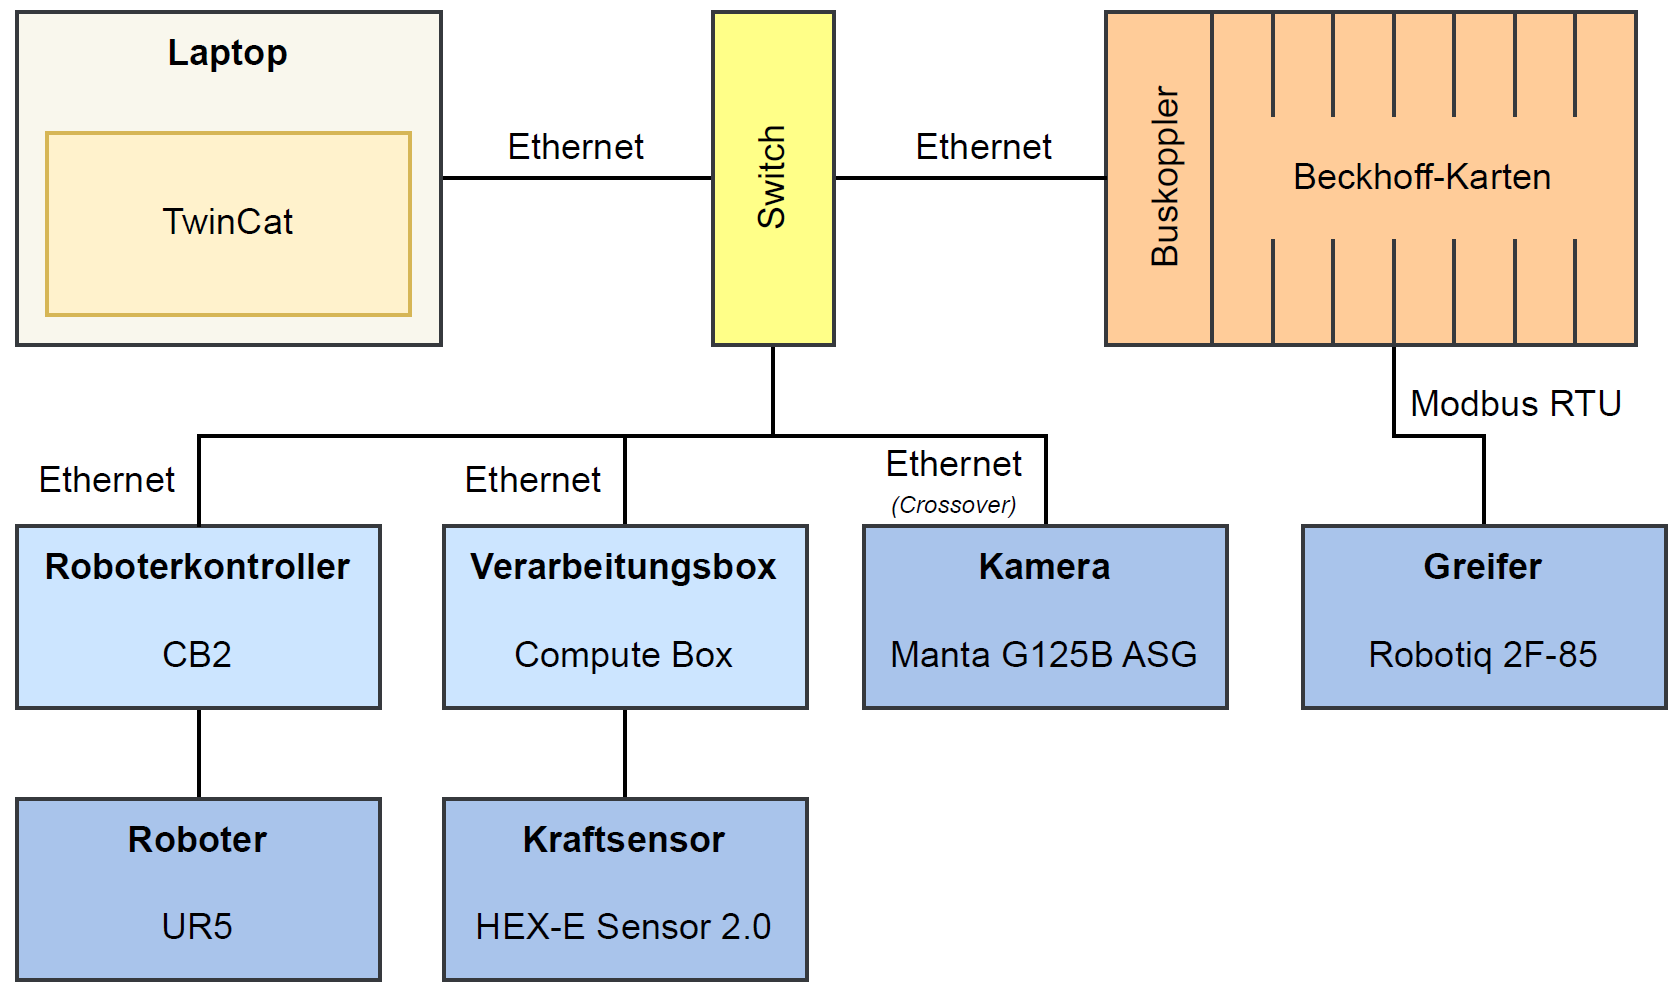
\includegraphics[width=0.8\textwidth]{04_Anwendung_und_Aufbau/Kommunikationstopologie}
		\captionsetup{justification=centering}
		\caption{Kommunikationstopologie}
		\label{fig:Kommunikationstopologie}
	\end{figure}
	
	Für die Umsetzung des Versuchsaufbaus wird ein Laptop mit TwinCAT als SPS eingesetzt. Der Grund dafür ist die Leistungsfähigkeit. Da alle Funktionalitäten innerhalb der SPS stattfinden sollen, muss diese auch die entsprechende Power mitbringen. 
	\\
	Die Switch verbindet den Laptop mit dem Bus-Koppler und den entsprechenden Komponenten der Prozesszelle. Teil des Netzwerkes ist der Roboterkontroller, die Signalverarbeitungsbox des Kraftsensors und die Kamera. 
	
	\textbf{Roboter und Roboterkontroller:}
	\vspace{2mm} 
	\\
	Der UR5-Roboter von Universal Robots wurde als Robotersystem ausgewählt. Dieser kollaborative Roboter zeichnet sich durch eine benutzerfreundliche Kommunikationsschnittstelle aus und kann schnell und unkompliziert in Betrieb genommen werden. An der BFH besteht umfassende Erfahrung mit dem UR5, und es stehen verschiedene Peripherie-Tools zur Verfügung.
	\\
	Mit einer Traglast von 5 kg und einer Reichweite von 850 mm ist der Roboter für vielfältige Anwendungen geeignet. Als Kommunikationsschnittstelle zwischen TwinCAT und Kontroller wird eine TCP/IP-Schnittstelle verwendet. Dafür muss TwinCAT mit dem TF6310-Paket (TwinCAT 3 TCP/IP) oder TF6311-Paket (TwinCAT 3 TCP/UDP Realtime) versehen werden, wobei TF6310 auch eine UDP-Kommunikation aufbauen kann. Bei TF6311 wird jedoch direkt über die Netzwerkkarte mit dem Server oder Client kommuniziert, was eine spezielle Hardwareschnittstelle voraussetzt. Diese Schnittstellen ermöglicht das Programmieren des Roboters über URScript. Der Kontroller verfügt aber auch über digitale und analoge Ein- und Ausgänge. 
	
	\textbf{Kamera:}
	\vspace{2mm} 
	\\
	Als Kamera kommt die „Manta G125B ASG“ zum Einsatz, die mit der weit verbreiteten GigE-Vision-Schnittstelle ausgestattet ist. Dadurch lässt sie sich direkt aus TwinCAT auslesen und konfigurieren. Um die Kamera in Betrieb zu nehmen, müssen die TF7XXX-Pakete (TwinCAT 3 Vision) installiert sein. Der Anschluss der Kamera erfolgt über eine Ethernet-Schnittstelle mithilfe eines Crossover-Kabels.
	
	\textbf{Kraftmessungssensor:}
	\vspace{2mm} 
	\vspace{-3mm} 
	\vspace{-\baselineskip}
	\vspace{-\baselineskip}
	\\
	\begin{wrapfigure}{r}{0.35\textwidth}
		\centering
		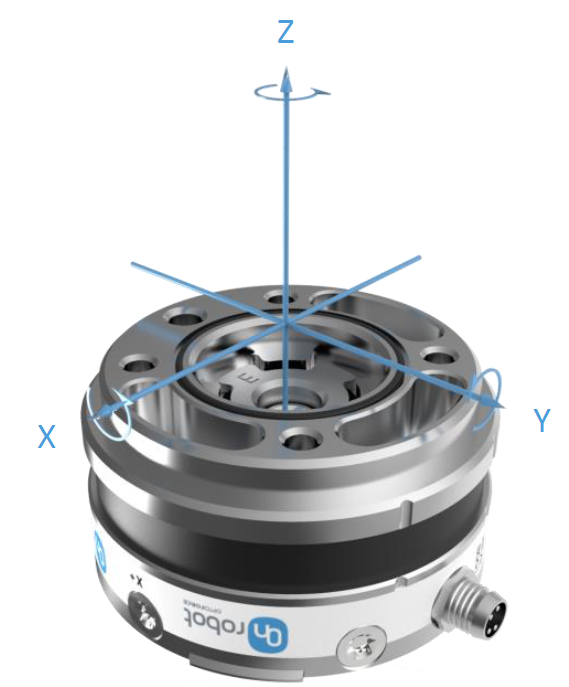
\includegraphics[width=0.35\textwidth]{04_Anwendung_und_Aufbau/Kraftsensor}
		\captionsetup{justification=centering}
		\caption{Kraftsensor}
		\label{fig:Kraft_sensor}
	\end{wrapfigure} \par
	Im Gegensatz zum UR5e verfügt der UR5 über keine integrierten Kraft-/Drehmomentsensoren in den Gelenken, was eine präzise Kraftregelung erschwert. Um dies zu kompensieren, kann der UR5 mit einem externen Kraftmesssensor ausgestattet werden. Hierfür eignet sich der „HEX-E Sensor 2.0“ von OnRobot (\ref{fig:Kraft_sensor}), der an der mechanischen Schnittstelle des UR5 montiert werden kann. 
	\\
	Der Sensor misst Kräfte und Drehmomente in und um drei Achsen. Die erfassten Daten werden an eine Signalverarbeitungsbox weitergeleitet, die das Rohsignal verarbeitet und über eine Ethernet-Schnittstelle zur Verfügung stellt. Die Kommunikation kann über eine UDP- oder TCP-Schnittstelle erfolgen. Für die Integration in TwinCAT kann das TF6310-Paket (TwinCAT 3 TCP/IP) verwendet.
	
	\textbf{Greifer:}
	\vspace{2mm} 
	\\
	Für das System wird der 2F-85-Greifer von Robotiq verwendet (\ref{fig:Greifer}), der speziell für die Integration mit UR-Robotern entwickelt wurde. Die Montage erfolgt einfach mittels einer Adapterplatte, und der Greifer wird direkt über den Anschluss am UR5-Roboter verbunden. Der eingesetzte CB2-Kontroller ist gerade noch in der Lage den Greifer betreiben zu können. 
	
	\begin{figure}[h!]
		\centering
		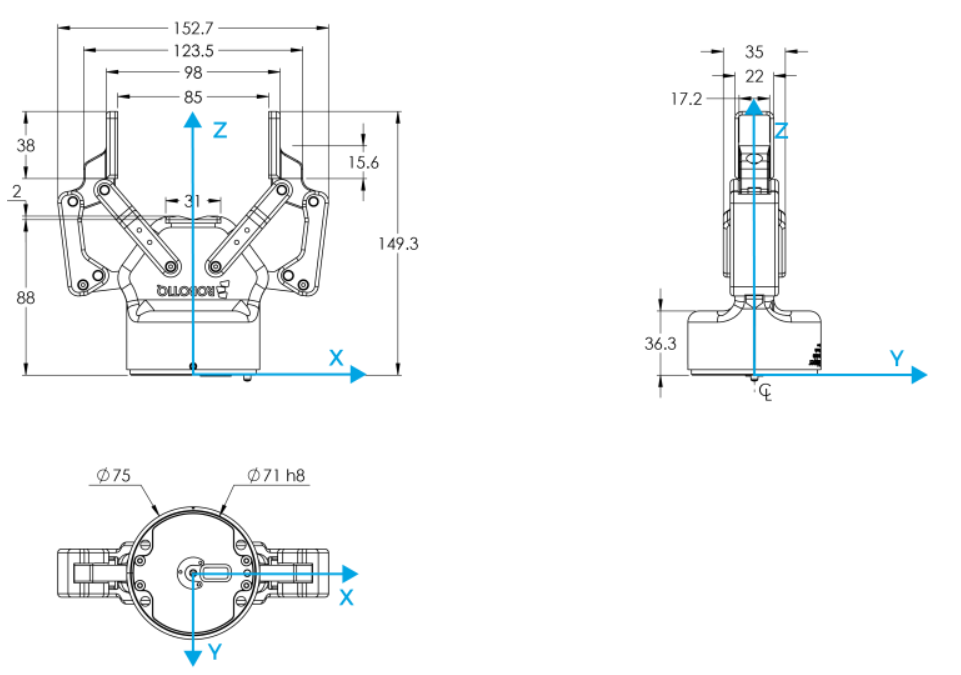
\includegraphics[width=1\textwidth]{04_Anwendung_und_Aufbau/Greifer}
		\captionsetup{justification=centering}
		\caption{Kommunikationstopologie}
		\label{fig:Greifer}
	\end{figure}
	
	Der 2F-85-Greifer bietet eine maximale Greifweite von 85 mm und wird elektrisch betrieben. Dank integrierter Sensoren lässt sich die Greifkraft präzise überwachen und anpassen. Auch die Fingerposition wird überwacht, was dem Greifer eine hohe Flexibilität in verschiedenen Anwendungen ermöglicht.